\documentclass[11pt]{article}
\usepackage[letterpaper,margin=0.82in,headheight=15pt]{geometry}
\usepackage[T1]{fontenc}
\usepackage[utf8]{inputenc}
\usepackage{lmodern}
\usepackage{microtype}
\usepackage{amsmath,amssymb,mathtools,bm,mathrsfs,amsthm}
\usepackage{booktabs,longtable,tabularx,array}
\usepackage{graphicx}
\usepackage{xcolor}
\usepackage{enumitem}
\usepackage{fancyhdr}
\usepackage{hyperref}
\usepackage[nameinlink,noabbrev]{cleveref}
\usepackage{tcolorbox}
\usepackage{titlesec}
\usepackage{float}
\usepackage{siunitx}
\usepackage{tikz}
\usetikzlibrary{arrows.meta,positioning,calc,fit,shapes.geometric}

\definecolor{ink}{HTML}{172033}
\definecolor{accent}{HTML}{345B83}
\definecolor{soft}{HTML}{EEF4F8}
\definecolor{result}{HTML}{ECF6EF}
\definecolor{warn}{HTML}{FAF3E8}
\definecolor{open}{HTML}{F3EFF8}
\definecolor{muted}{HTML}{5A6472}
\hypersetup{colorlinks=true,linkcolor=accent,citecolor=accent,urlcolor=accent,
  pdftitle={Causal-Wall Spectral Theory: A Non-Stochastic Spectral Formulation of the Scalar Cosmological Sector},
  pdfauthor={Thomas Ruble}}
\pagestyle{fancy}
\fancyhf{}
\lhead{Causal-Wall Spectral Theory}
\rhead{Technical memorandum v3.0}
\cfoot{\thepage}
\setlength{\parindent}{0pt}
\setlength{\parskip}{0.53em}
\setlist[itemize]{topsep=0.25em,itemsep=0.16em,leftmargin=1.6em}
\setlist[enumerate]{topsep=0.25em,itemsep=0.18em,leftmargin=1.75em}
\titleformat{\section}{\Large\bfseries\color{ink}}{\thesection}{0.65em}{}
\titleformat{\subsection}{\large\bfseries\color{ink}}{\thesubsection}{0.6em}{}
\numberwithin{equation}{section}

\newcommand{\dd}{\mathrm d}
\newcommand{\ii}{\mathrm i}
\newcommand{\BKM}{\mathrm{BKM}}
\newcommand{\Tr}{\operatorname{Tr}}
\newcommand{\Disc}{\operatorname{Disc}}
\newcommand{\Sc}{\mathfrak{Sc}}
\newcommand{\Wall}{\mathfrak W}
\newcommand{\Iz}{\mathcal I_\zeta}
\newcommand{\Kz}{\mathcal K_\zeta}
\newcommand{\Gz}{\mathcal G_\zeta}
\newcommand{\Cz}{\mathcal C_\zeta}
\newcommand{\cz}{c^{(0)}}
\newcommand{\ct}{c^{(2)}}
\newcommand{\Sfrak}{\mathfrak S}
\newcommand{\Order}{\mathcal O}
\newcommand{\status}[1]{\textsc{\footnotesize #1}}
\newcolumntype{Y}{>{\raggedright\arraybackslash}X}

\newtcolorbox{thesisbox}{colback=soft,colframe=accent,boxrule=0.8pt,arc=1.2mm,left=3mm,right=3mm,top=2mm,bottom=2mm}
\newtcolorbox{resultbox}{colback=result,colframe=green!45!black,boxrule=0.8pt,arc=1.2mm,left=3mm,right=3mm,top=2mm,bottom=2mm}
\newtcolorbox{warningbox}{colback=warn,colframe=orange!55!black,boxrule=0.7pt,arc=1.2mm,left=3mm,right=3mm,top=2mm,bottom=2mm}
\newtcolorbox{openproblembox}{colback=open,colframe=purple!45!black,boxrule=0.7pt,arc=1.2mm,left=3mm,right=3mm,top=2mm,bottom=2mm}

\newtheorem{theorem}{Theorem}[section]
\newtheorem{proposition}[theorem]{Proposition}
\newtheorem{lemma}[theorem]{Lemma}
\theoremstyle{definition}
\newtheorem{definition}[theorem]{Definition}
\theoremstyle{remark}
\newtheorem{remark}[theorem]{Remark}

\begin{document}
\hypersetup{pageanchor=false}
\begin{titlepage}
\thispagestyle{empty}
\centering
\vspace*{0.42in}
{\Huge\bfseries\color{ink} Causal-Wall Spectral Theory\par}
\vspace{0.18in}
{\LARGE A Non-Stochastic Spectral Formulation of the\par}
\vspace{0.06in}
{\LARGE Scalar Cosmological Sector\par}
\vspace{0.42in}
{\Large Technical memorandum v3.0\par}
\vspace{0.52in}
{\large Thomas Ruble research programme\par}
\vspace{0.10in}
{\normalsize 22 August 2026\par}
\vfill
\begin{minipage}{0.93\textwidth}
\small
\textbf{Status.} Working research memorandum; not peer reviewed. This revision integrates and audits the v2.0 referee recommendations. It separates four registers that the earlier draft partly compressed: (i) an exact Fourier and holographic spectral dictionary; (ii) a conditional information-geometric lemma for regular Weyl-source families; (iii) a minimal near-critical power-law member; and (iv) the still-open causal-wall construction that must identify the actual algebra, state, and scale-to-state map. The title has been weakened from ``completion'' to ``formulation'' because the microscopic weld has not yet been proved. A factor-of-two normalization hidden in v2.0 is repaired by using the symmetrized relative entropy, equivalently twice the one-sided BKM Hessian. No ontological random field or temporally localized stochastic seeding event is assumed.
\end{minipage}
\end{titlepage}
\hypersetup{pageanchor=true}
\setcounter{page}{1}

\begin{abstract}
The cosmic microwave background constrains a hierarchy of correlations; it does not decide whether those correlations were generated by primitive stochastic events. This memorandum formulates the scalar sector as a spectral problem for a wall-relative logarithmic scale residue $\zeta=-\delta\ln\sigma$. The observable quadratic datum is the positive precision kernel of $\zeta$, whose inverse is its covariance.

For a regular quantum exponential family generated by the wall stress trace, the Hessian of the \emph{symmetrized} relative entropy is twice the BKM metric. After spectral continuation, this factor of two is exactly the factor acquired when a wavefunctional is converted to a probability weight. Under that conditional source-family hypothesis,
\[
\Kz(k)=8\,\rho_B(k),
\qquad
\rho_B(k):=\operatorname{Im}B(-k^2-\ii0)\ge0.
\]
Together with the established holographic dictionary,
\[
\Delta_\zeta^2(k)=\frac{k^3}{16\pi^2\rho_B(k)}
=\frac{4}{\pi^4\cz(k)},
\]
this gives
\[
\boxed{
\Kz(k)=\frac{\pi^2}{8}\cz(k)k^3
=\frac{\Iz(k)}{2\pi^2}k^3,
\qquad
\Iz(k)=\frac{\pi^4}{4}\cz(k)=\frac1{\Delta_\zeta^2(k)}.}
\]
Local analytic contact terms vanish under the discontinuity across the spectral cut.

Homogeneity, isotropy, a dimensionless scalar, positivity, and exact dilation covariance force the flat critical shape $|k|^3$. Given a suitable conformal filling, its canonical scattering-theoretic curved representative is the fractional GJMS operator $P_3$. The physical trace response nevertheless vanishes at an exact conformal fixed point: $P_3$ specifies the \emph{shape} of the near-critical kernel, while its coefficient tends to zero as $T=\beta^I\Order_I\to0$. At that point the precision operator is degenerate and must be quotiented before inversion; a formally divergent inverse is not a physical prediction of infinite lumpiness.

The observed red tilt is the running of inverse scalar power,
\[
n_s-1=-\frac{\dd\ln\Iz}{\dd\ln k},
\qquad
\alpha_s=-\frac{\dd^2\ln\Iz}{\dd(\ln k)^2}.
\]
A constant-exponent power law is one economical member and predicts $\alpha_s=0$ by definition; the general spectral typing does not supply a universal next-order bound without a microscopic beta function. Planck 2018 fixes $\Iz(k_*)=4.764\times10^8$ and $\cz(k_*)=1.956\times10^7$ at $k_*=0.05\,\mathrm{Mpc}^{-1}$. The BK18 bound $r<0.036$, with the registered tensor normalization, gives $\ct/\cz>222.2$ and a per-polarization precision ratio $\mathcal K_\gamma/\Kz>55.6$.

Rank-one descent conditionally yields adiabaticity, superhorizon conservation, and passive coherent transfer. Higher-point predictions require the cubic and higher wavefunctional vertices derived from $\langle TTT\rangle$ and semilocal terms; they are not obtained by identifying higher derivatives of relative entropy directly with connected cosmological cumulants. The outstanding theorem is therefore sharp: construct the causal-wall algebra and state, prove the Weyl-source/BKM spectral weld, and compute $\cz(k)$, $\ct(k)$, and the higher stress correlators. The result is a non-stochastic formulation with a finite research target, not yet a microscopic completion.
\end{abstract}

\tableofcontents
\clearpage

\section{Empirical target and claim registers}

The conventional sentence ``quantum fluctuations perturb an initially homogeneous universe'' combines three distinct claims:
\begin{enumerate}
\item a homogeneous FLRW presentation is used as a zeroth-order metric;
\item the observable state has nonzero connected correlations around that presentation;
\item those correlations are represented by a classical random field in a useful calculational model.
\end{enumerate}
Only the first two are demanded by the data. The third does not, by itself, establish primitive ontological chance.

The scalar sector must provide
\begin{equation}
\boxed{
\text{two-point shape and amplitude, mode content, phase coherence, higher cumulants, and transfer laws}.}
\end{equation}
It need not provide a temporally localized random kick.

\begin{thesisbox}
\textbf{Retyped target.} The leading scalar object is the positive precision operator of the wall-relative logarithmic scale residue. A random field is one commutative representation of the inverse covariance; it is not part of the primitive ontology asserted here.
\end{thesisbox}

The argument uses four claim registers:
\begin{center}
\begin{tabularx}{0.94\textwidth}{@{}p{0.18\textwidth}Y@{}}
\toprule
\textbf{Register} & \textbf{Meaning in this memorandum}\\
\midrule
\status{Established} & A theorem or published dictionary, once its assumptions and normalization are fixed.\\
\status{Conditional} & A derivation inside a stated member, regularization, or source-family hypothesis.\\
\status{Programme hypothesis} & A proposed identification that the causal-wall construction must prove.\\
\status{Open slot} & A quantity whose mathematical type is fixed but whose value or function is not yet computed.\\
\bottomrule
\end{tabularx}
\end{center}

\begin{remark}[Register discipline for cosmic time]
If the pre-observable structure is not itself a Lorentzian metric state, it need not be parameterized by FLRW proper time. This is an agnostic statement about the ontology of the reconstruction, not a new empirical claim about the age of the universe.
\end{remark}

\section{Scale residue, covariance, and precision}

Let $\Sigma$ be an observable spatial wall and let $\Sc(\Sigma)$ be the groupoid of positive scale sections
\begin{equation}
\sigma\in\Gamma(\mathcal E[1]),\qquad \sigma>0,
\end{equation}
with changes of conformal trivialization as morphisms. Around a homogeneous reference $\bar\sigma$, write
\begin{equation}
-\delta\ln\sigma(x)=\delta N+\zeta(x).
\end{equation}
Here $\delta N$ is the homogeneous scale displacement and $\zeta$ is the inhomogeneous residue. On a compact wall one may impose $\int_\Sigma\zeta=0$; in flat space one removes the $k=0$ mode. Thus
\begin{equation}
T_{\bar\sigma}\Sc(\Sigma)
\simeq \mathbb R\oplus C^\infty(\Sigma)/\mathbb R.
\end{equation}
The quotient separates background clock displacement from inhomogeneity. It does not, by itself, prove orthogonality in an arbitrary information metric; that issue is returned to in \cref{sec:CSD}.

Fix Fourier conventions by
\begin{equation}
\langle\zeta_{\bm k}\zeta_{\bm k'}\rangle
=(2\pi)^3\delta^{(3)}(\bm k+\bm k')P_\zeta(k),
\qquad
\Delta_\zeta^2(k)=\frac{k^3}{2\pi^2}P_\zeta(k).
\end{equation}
If the quadratic probability weight is
\begin{equation}
\mathbb P[\zeta]\propto
\exp\!\left[-\frac12\int\frac{\dd^3k}{(2\pi)^3}
\Kz(k)|\zeta_{\bm k}|^2\right],
\end{equation}
then
\begin{equation}
P_\zeta(k)=\Kz(k)^{-1},
\qquad
\boxed{\Kz(k)=\frac{k^3}{2\pi^2\Delta_\zeta^2(k)}.}
\label{eq:precision-definition}
\end{equation}
This identity is purely probabilistic and fixes all later factors.

\section{The information-geometric weld, with its assumptions exposed}
\label{sec:weld}

Let $\Wall$ denote a proposed stack of observer-dressed walls carrying a local algebra $\mathcal A_\Sigma$, a faithful state $\omega_\Sigma$, modular comparison data, and scale geometry. The programme seeks a scale-to-state map
\begin{equation}
\Phi:\Sc(\Sigma)\longrightarrow\Wall,
\qquad
\omega_{\Sigma,\zeta}=\Phi(\bar\sigma e^{-\zeta}).
\end{equation}
The following finite or suitably regularized lemma is exact. Its realization by the actual continuum wall state is an open theorem.

\subsection{Why the symmetrized relative entropy is the correct normalization}

\begin{proposition}[Exponential-family Hessian]
Let
\begin{equation}
\rho_\zeta
=\exp\!\left(\log\rho_0+X[\zeta]-\psi[\zeta]\right),
\qquad
X[\zeta]=\int_\Sigma\sqrt g\,\zeta(x)T(x),
\end{equation}
be a regular quantum exponential family, with $\psi$ chosen to normalize the state. At $\zeta=0$,
\begin{align}
\operatorname{Hess}D(\rho_\zeta\|\rho_0)&=G^{\BKM},\\
\operatorname{Hess}D(\rho_0\|\rho_\zeta)&=G^{\BKM}.
\end{align}
Therefore the symmetrized divergence
\begin{equation}
\mathscr J[\zeta]
:=D(\rho_\zeta\|\rho_0)+D(\rho_0\|\rho_\zeta)
\end{equation}
has Hessian
\begin{equation}
\boxed{
\left.\frac{\delta^2\mathscr J}{\delta\zeta(x)\delta\zeta(y)}\right|_0
=2G^{\BKM}_{TT}(x,y).}
\label{eq:sym-bkm}
\end{equation}
\end{proposition}

\begin{proof}
For an exponential family, $D(\rho_\zeta\|\rho_0)$ is the Bregman remainder of $\psi$ in one orientation, while $D(\rho_0\|\rho_\zeta)$ is the reverse Bregman remainder. Both have the same quadratic term, the Kubo--Mori/Bogoliubov metric. Their sum therefore has twice that Hessian. In the commuting limit this is twice the Fisher covariance of the score $T$.
\end{proof}

This repairs a normalization hidden in v2.0. The one-sided relative-entropy Hessian is one BKM metric, whereas the cosmological probability precision is twice the continued wavefunctional kernel because $|\Psi|^2$ doubles the real suppression exponent. One may equivalently retain one-sided relative entropy and define the cosmological precision as twice its Hessian. We use the symmetric form because it keeps the geometric and probability normalizations in one object.

\begin{warningbox}
\textbf{Conditional joint.} The first Weyl variation of a generating functional does not, by itself, prove that the physical map $\Phi$ is a quantum exponential family generated by $T$. The programme must construct the relevant Araki/cocycle-perturbed family in the wall algebra and prove the required regularity. Equation \eqref{eq:sym-bkm} states what follows \emph{if} that joint is established.
\end{warningbox}

\subsection{Weyl sources, stress trace, and contact terms}

Let $W_\Sigma[g]=\log Z_\Sigma[g]$ be the Euclidean connected generating functional. For a local Weyl source $g_{ij}\mapsto e^{2\zeta}g_{ij}$,
\begin{equation}
\frac{\delta W_\Sigma}{\delta\zeta(x)}
=\sqrt g\,\langle T^i{}_i(x)\rangle
\end{equation}
up to the registered overall source sign. A second variation gives the connected trace response plus local terms,
\begin{equation}
\frac{\delta^2 W_\Sigma}{\delta\zeta(x)\delta\zeta(y)}
=\langle T(x)T(y)\rangle_c+\text{local contacts}.
\end{equation}
For a three-dimensional QFT, decompose
\begin{equation}
\langle\!\langle T_{ij}(q)T_{kl}(-q)\rangle\!\rangle
=A(q^2)\Pi_{ijkl}+B(q^2)\pi_{ij}\pi_{kl},
\end{equation}
so that
\begin{equation}
\langle\!\langle T(q)T(-q)\rangle\!\rangle=4B(q^2).
\end{equation}
Define the positive spectral discontinuities
\begin{equation}
\rho_B(k):=\frac{1}{2\ii}\Disc B(-k^2)
=\operatorname{Im}B(-k^2-\ii0)\ge0,
\end{equation}
\begin{equation}
\rho_A(k):=\frac{1}{2\ii}\Disc A(-k^2)
=\operatorname{Im}A(-k^2-\ii0)\ge0.
\end{equation}
Local counterterms are polynomial, hence analytic, in $q^2$. Therefore
\begin{equation}
\Disc p(q^2)=0
\end{equation}
for every local polynomial $p$, and the spectral discontinuity is precisely the quotient by local contact ambiguity.

On a closed odd-dimensional wall there is no ordinary local bulk Weyl anomaly. Boundaries, defects, and parity-odd local terms require their own bookkeeping, but none contributes to the parity-even scalar spectral discontinuity used below.

Under the source-family condition of the preceding subsection, the spectral part of the standard BKM Hessian is $4\rho_B$. The symmetrized Hessian is therefore
\begin{equation}
\boxed{\Kz(k)=8\rho_B(k).}
\label{eq:weld}
\end{equation}
This is the desired weld. It is exact once the source-family hypothesis and continuation convention are established; constructing them for the causal wall is \status{open}.

\section{The exact holographic spectral dictionary}
\label{sec:dictionary}

McFadden and Skenderis derive the scalar and tensor spectra from the continued stress-tensor response:
\begin{equation}
\boxed{
\Delta_S^2(k)=\frac{k^3}{16\pi^2\rho_B(k)},
\qquad
\Delta_T^2(k)=\frac{2k^3}{\pi^2\rho_A(k)}.}
\label{eq:MS}
\end{equation}
Introduce nonnegative spin-zero and spin-two spectral densities by the registered normalizations
\begin{equation}
\rho_B(k)=\frac{\pi^2}{64}\cz(k)k^3,
\qquad
\rho_A(k)=\frac{\pi^2}{16}\ct(k)k^3.
\label{eq:c-normalizations}
\end{equation}
Then
\begin{equation}
\boxed{
\Delta_S^2(k)=\frac{4}{\pi^4\cz(k)},
\qquad
\Delta_T^2(k)=\frac{32}{\pi^4\ct(k)}.}
\label{eq:holo-powers}
\end{equation}
Combining \cref{eq:precision-definition,eq:holo-powers} gives, without any further physics,
\begin{equation}
\boxed{
\Kz(k)=\frac{\pi^2}{8}\cz(k)k^3.}
\end{equation}
Define scalar discernibility
\begin{equation}
\boxed{\Iz(k):=\frac{\pi^4}{4}\cz(k)=\frac{1}{\Delta_\zeta^2(k)}.}
\end{equation}
The central dictionary is therefore
\begin{equation}
\boxed{
\Kz(k)
=8\rho_B(k)
=\frac{\pi^2}{8}\cz(k)k^3
=\frac{\Iz(k)}{2\pi^2}k^3.}
\label{eq:main-dictionary}
\end{equation}

\begin{figure}[H]
\centering
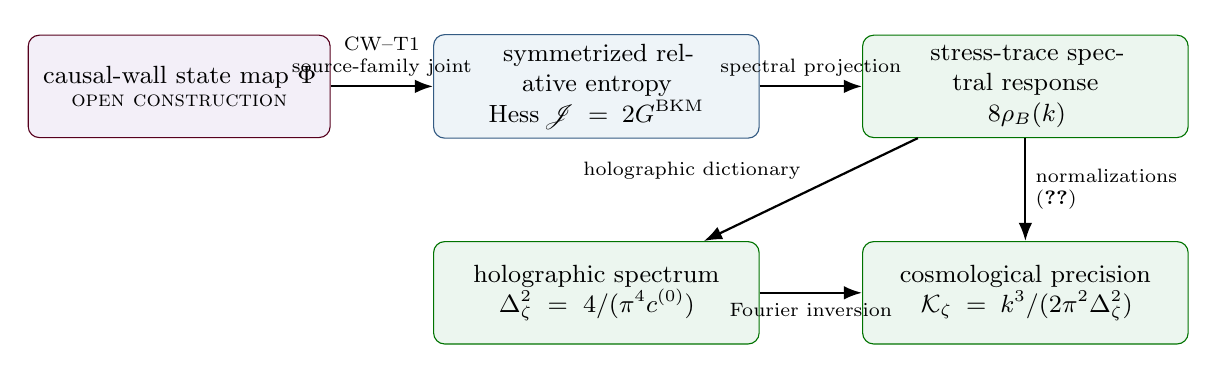
\begin{tikzpicture}[node distance=13mm and 13mm,>=Latex,font=\small,
  box/.style={draw=accent,rounded corners,fill=soft,align=center,text width=39mm,minimum height=13mm},
  exact/.style={draw=green!45!black,rounded corners,fill=result,align=center,text width=39mm,minimum height=13mm},
  openstyle/.style={draw=purple!45!black,rounded corners,fill=open,align=center,text width=36mm,minimum height=13mm}]
\node[openstyle] (wall) {causal-wall state map $\Phi$\\[-1mm]{\scriptsize\status{open construction}}};
\node[box,right=of wall] (bkm) {symmetrized relative entropy\\$\operatorname{Hess}\mathscr J=2G^{\BKM}$};
\node[exact,right=of bkm] (trace) {stress-trace spectral response\\$8\rho_B(k)$};
\node[exact,below=of bkm] (spec) {holographic spectrum\\$\Delta_\zeta^2=4/(\pi^4\cz)$};
\node[exact,right=of spec] (cosmo) {cosmological precision\\$\Kz=k^3/(2\pi^2\Delta_\zeta^2)$};
\draw[->,thick] (wall) -- node[above,font=\scriptsize,align=center]{CW--T1\\source-family joint} (bkm);
\draw[->,thick] (bkm) -- node[above,font=\scriptsize]{spectral projection} (trace);
\draw[->,thick] (trace) -- node[right,font=\scriptsize,align=left]{normalizations\\\eqref{eq:c-normalizations}} (cosmo);
\draw[->,thick] (trace) -- node[above left,font=\scriptsize]{holographic dictionary} (spec);
\draw[->,thick] (spec) -- node[below,font=\scriptsize]{Fourier inversion} (cosmo);
\end{tikzpicture}
\caption{Two routes to scalar precision. The spectral and Fourier arrows are established once conventions are fixed. The first arrow---construction of the causal-wall source family---is the programme's load-bearing open theorem.}
\end{figure}

The term \emph{precision} refers to $\Kz$; \emph{discernibility} to $\Iz$; \emph{scalar response} to $\cz$; and \emph{spin-two capacity} to $\ct$ (or the fixed-point $c_T$ scale when such an identification is justified). These words are not interchangeable.

\section{Critical shape and the conformal operator $P_3$}
\label{sec:P3}

\subsection{Flat-space uniqueness}

Assume:
\begin{enumerate}
\item a homogeneous and isotropic three-dimensional wall;
\item a dimensionless weight-zero scalar residue $\zeta$;
\item a positive translation-invariant quadratic form;
\item exact dilation covariance and no intrinsic scale in the critical member.
\end{enumerate}
Then
\begin{equation}
\mathscr J^{(2)}[\zeta]
=\frac12\int\frac{\dd^3k}{(2\pi)^3}\Kz(k)|\zeta_{\bm k}|^2.
\end{equation}
Under $x\mapsto\lambda x$, a dimensionless scalar has $\zeta_{\bm k}\mapsto\lambda^3\zeta_{\lambda\bm k}$, and invariance requires
\begin{equation}
\Kz(\lambda k)=\lambda^3\Kz(k).
\end{equation}
Isotropy and positivity therefore give
\begin{equation}
\boxed{\Kz(k)=C|k|^3,\qquad C\ge0.}
\label{eq:k3}
\end{equation}
The inverse covariance has the scale-invariant shape $k^{-3}$ whenever $C>0$.

\subsection{Curved completion and what it does not prove}

Given a conformal three-manifold $(\Sigma,[g])$ and a suitable Poincar\'e--Einstein or scattering filling, the canonical scattering construction yields the critical fractional GJMS operator $P_3^g$, with
\begin{equation}
P_3=(-\Delta)^{3/2}
\end{equation}
in flat space. This is the natural conformally covariant completion of \eqref{eq:k3} \emph{relative to the filling data}. Flat symmetry alone does not prove uniqueness of a curved nonlocal operator on every conformal manifold without specifying such global data.

On a round three-sphere of radius $R$,
\begin{equation}
\boxed{
P_3Y_{\ell mn}
=R^{-3}\ell(\ell+1)(\ell+2)Y_{\ell mn},
\qquad \ell\ge1.}
\end{equation}
The constant mode lies in the kernel, matching the removal of the homogeneous residue.

\begin{resultbox}
\textbf{What is fixed.} The critical \emph{shape} of a dimensionless scalar precision kernel is $P_3$. The overall coefficient and its running are dynamical spectral data. The actual causal-wall construction must still show that its relative-entropy Hessian lands in this conformal class.
\end{resultbox}

\section{The fixed-point degeneracy and controlled flow}
\label{sec:fixedpoint}

At a conformal fixed point, after improvement and away from anomalies,
\begin{equation}
T=0.
\end{equation}
Along a controlled deformation,
\begin{equation}
T=\beta^I(g)\Order_I
\end{equation}
up to improvement and contact terms, so schematically
\begin{equation}
\langle TT\rangle
\sim \beta^I\beta^J\langle\Order_I\Order_J\rangle.
\end{equation}
Consequently the spin-zero response vanishes as the flow approaches the fixed point:
\begin{equation}
\cz(k)\longrightarrow0,
\qquad
\Kz\longrightarrow0.
\end{equation}
This does \emph{not} mean that the fixed point predicts infinite observable lumpiness. It means that the Weyl-source direction has become null or redundant in state space. The inverse $\Kz^{-1}$ does not exist on that direction. One must first quotient the null direction or pass to gauge-invariant observables; only then is inversion meaningful.

This resolves the apparent contradiction between ``scale is gauge'' and the formal expression $\Delta_\zeta^2=1/\Iz$. The latter is valid only where $\Iz>0$ and $\zeta$ is a physical coordinate. The exact fixed point is a singular chart boundary for the scalar clock variable, analogous to the $\epsilon\to0$ degeneracy of the comoving curvature variable in exact de Sitter space.

The correct near-critical form is therefore
\begin{equation}
\Kz\simeq C(k)P_3,
\qquad
C(k)=\frac{\pi^2}{8}\cz(k),
\end{equation}
with $C(k)$ small or slowly varying according to the microscopic deformation. $P_3$ describes the normalized critical shape; it is not a nonzero trace operator at the exact fixed point.

Two independent statements must be kept separate:
\begin{enumerate}
\item \textbf{shape near criticality:} $|\dd\ln\cz/\dd\ln k|\ll1$;
\item \textbf{small scalar power:} $\Iz\gg1$.
\end{enumerate}
The measured value of $\cz$ is a convention-dependent spin-zero response, not by itself a fixed-point central charge. In particular, no effective rank $N\sim\sqrt{\cz}$ may be inferred without a specified microscopic theory and normalization.

\begin{thesisbox}
\textbf{Explanatory sentence.} Structure exists because local scale is not exactly redundant; its faintness is large discernibility $\Iz$; its redness is the slow running of that discernibility.
\end{thesisbox}

\section{Tilt, running, and the minimal power-law member}
\label{sec:tilt}

From \cref{eq:main-dictionary},
\begin{equation}
\Delta_\zeta^2(k)=\Iz(k)^{-1}.
\end{equation}
Hence the spectral index and running satisfy the exact identities
\begin{equation}
\boxed{
n_s(k)-1
=\frac{\dd\ln\Delta_\zeta^2}{\dd\ln k}
=-\frac{\dd\ln\Iz}{\dd\ln k}
=-\frac{\dd\ln\cz}{\dd\ln k},}
\label{eq:tilt}
\end{equation}
\begin{equation}
\boxed{
\alpha_s(k):=\frac{\dd n_s}{\dd\ln k}
=-\frac{\dd^2\ln\Iz}{\dd(\ln k)^2}.}
\label{eq:running}
\end{equation}

The minimal power-law member assumes
\begin{equation}
\cz(k)=\cz_*
\left(\frac{k}{k_*}\right)^{\delta},
\qquad
\delta=1-n_s=\text{constant}.
\end{equation}
It follows that
\begin{equation}
\Delta_\zeta^2(k)=A_s
\left(\frac{k}{k_*}\right)^{-\delta},
\qquad
\boxed{\alpha_s=0.}
\end{equation}
This is an exact prediction of that \emph{member}, because constant $\delta$ defines the member. The general spectral formulation has not derived a universal estimate such as $|\alpha_s|\lesssim\delta^2$; obtaining one requires a concrete beta function or other microscopic flow law.

The quoted data summaries are:
\begin{center}
\begin{tabular}{@{}lccc@{}}
\toprule
\textbf{Combination} & $n_s$ & $\delta=1-n_s$ & \textbf{Interpretation}\\
\midrule
Planck 2018 baseline & $0.9649\pm0.0042$ & $0.0351\pm0.0042$ & one data/model summary\\
P--ACT alone & $0.9709\pm0.0038$ & $0.0291\pm0.0038$ & different combination\\
P--ACT--LB & $0.9743\pm0.0034$ & $0.0257\pm0.0034$ & adds lensing and DESI BAO\\
\bottomrule
\end{tabular}
\end{center}
The Planck and P--ACT--LB central values differ by $0.0094$, or about $1.74\sigma$ if their quoted errors are combined naively. That number is a useful \status{watch item}, but it is not a measurement of running: the estimates arise from different likelihood combinations and weight overlapping scales differently. Converting their difference into $\alpha_s$ by assigning an ad hoc lever arm is not statistically valid. A joint extended-model likelihood is the appropriate test. The ACT DR6 extended-model analysis reports
\begin{equation}
\alpha_s=0.0062\pm0.0052,
\end{equation}
consistent with zero. A robust nonzero running would reject the constant-exponent member while leaving the broader spectral formulation intact.

The wall momentum $k$ is identified, in the holographic dictionary, with comoving cosmological wavenumber and simultaneously plays the role of a wall resolution/RG coordinate. Only dimensionless ratios such as $k/k_*$ enter the power-law member.

\section{Numerical scalar calibration}
\label{sec:calibration}

Fix the pivot
\begin{equation}
k_*=0.05\ \mathrm{Mpc}^{-1}.
\end{equation}
Using Planck's
\begin{equation}
\ln(10^{10}A_s)=3.044
\end{equation}
gives
\begin{equation}
A_s=2.098903\times10^{-9},
\end{equation}
\begin{equation}
\boxed{\Iz(k_*)=A_s^{-1}=4.764393\times10^8,}
\end{equation}
\begin{equation}
\boxed{\cz(k_*)=\frac{4}{\pi^4A_s}=1.956447\times10^7.}
\end{equation}
These are the scalar discernibility and spin-zero response in the normalization of \cref{eq:c-normalizations}; they are readings at a specified pivot, not constants of nature.

For a constant exponent, the multiplicative growth of discernibility per e-fold of $k$ is $e^\delta-1$:
\begin{equation}
3.57\%\quad\text{for }\delta=0.0351,
\qquad
2.60\%\quad\text{for }\delta=0.0257.
\end{equation}
The numerical calibration determines the target a microscopic wall theory must reproduce. It does not derive the value from the causal-wall algebra.

\section{Tensor slot and the Einstein single-clock member}
\label{sec:tensor}

The tensor spectral density in \cref{eq:holo-powers} is independent of the scalar response. At a common pivot,
\begin{equation}
\boxed{r:=\frac{\Delta_T^2}{\Delta_S^2}
=8\frac{\cz}{\ct}.}
\label{eq:r}
\end{equation}
The BK18 bound $r<0.036$ implies
\begin{equation}
\boxed{\frac{\ct}{\cz}>222.2,}
\qquad
\boxed{\ct(k_*)>4.35\times10^9.}
\end{equation}
These are spectral-density ratios. If $\Delta_T^2$ includes both tensor polarizations, the precision of one polarization is
\begin{equation}
\mathcal K_\gamma(k)=\frac{k^3}{\pi^2\Delta_T^2(k)},
\end{equation}
so that
\begin{equation}
\boxed{\frac{\mathcal K_\gamma}{\Kz}=\frac{2}{r}>55.6.}
\end{equation}
Thus ``more than two orders of magnitude'' applies to $\ct/\cz$, not to the per-polarization precision ratio.

The general spectral formulation leaves $\ct(k)$ as an \status{open slot}. It therefore does not yet predict $r$ or a universal tensor tilt.

\subsection{Conditional Einstein reconstruction}

In the leading semiclassical Einstein single-clock member, define
\begin{equation}
\Sfrak:=\frac{8\pi^2M_{\mathrm P}^2}{H^2}
=\frac{\pi}{GH^2},
\end{equation}
where $M_{\mathrm P}^{-2}=8\pi G$. The leading scalar and tensor spectra are
\begin{equation}
\Delta_\zeta^2=\frac{1}{\epsilon\Sfrak},
\qquad
\Delta_T^2=\frac{16}{\Sfrak}.
\end{equation}
Comparison with \cref{eq:holo-powers} gives
\begin{equation}
\boxed{
\cz=\frac{4\epsilon\Sfrak}{\pi^4},
\qquad
\ct=\frac{2\Sfrak}{\pi^4},
\qquad
\Iz=\epsilon\Sfrak.}
\label{eq:Einstein-member}
\end{equation}
At this order,
\begin{equation}
r=16\epsilon,
\qquad
n_t=-2\epsilon=-\frac r8.
\end{equation}
These are leading single-clock consistency relations, not exact identities of the general wall class.

The BK18 bound conditionally gives
\begin{equation}
\epsilon<2.25\times10^{-3},
\end{equation}
\begin{equation}
\Sfrak>\frac{16\Iz}{r}>2.118\times10^{11},
\end{equation}
\begin{equation}
H<4.70\times10^{13}\ \mathrm{GeV}.
\end{equation}
Their agreement with the independent Einstein-member calculation is a valuable normalization check. They are properties of this metric reconstruction, not evidence that the early state must be ontologically described as an inflationary spacetime.

\section{Rank one, conservation, and coherent transfer}
\label{sec:transfer}

The spectral dictionary alone does not imply adiabaticity. Add the \status{rank-one member hypothesis}: every separately conserved material sector is evaluated at the same local scale reading,
\begin{equation}
\rho_i(x)=\bar\rho_i(N+\zeta(x)).
\end{equation}
At linear order,
\begin{equation}
\delta\rho_i=\bar\rho_i'\zeta,
\end{equation}
so all species share the same curvature/clock residue and the relative entropy modes vanish,
\begin{equation}
\boxed{S_{ij}=3(\zeta_i-\zeta_j)=0.}
\end{equation}
Equivalently, the non-adiabatic pressure perturbation vanishes. Stress-energy conservation then gives the standard superhorizon relation
\begin{equation}
\frac{\dd\zeta}{\dd N}
=-\frac{\delta p_{\mathrm{nad}}}{\rho+p}
+\Order\!\left(\frac{k^2}{a^2H^2}\right),
\end{equation}
so $\zeta$ is conserved at leading gradient order.

That conservation law is the missing bridge between the wall covariance and the transfer integral at re-entry. Once the initial covariance is fixed,
\begin{equation}
C_\ell^{XY}
=4\pi\int\dd\ln k\,
\Delta_\zeta^2(k)\Theta_\ell^X(k)\Theta_\ell^Y(k).
\end{equation}
If no continuously active incoherent source is added, standard photon--baryon, neutrino, and gravitational transfer preserves acoustic phase coherence. Thus one hypothesis---rank-one passive descent---yields adiabaticity, superhorizon conservation, and coherent transfer. These are conditional consequences of the member, not theorems of an arbitrary wall QFT.

\section{Higher-point functions without a covariance--vertex conflation}
\label{sec:higher}

The v2.0 shorthand
\[
K_3\leftrightarrow\text{bispectrum},
\qquad
K_4\leftrightarrow\text{trispectrum}
\]
is too compressed. Three distinct objects must be separated:
\begin{enumerate}
\item derivatives of a source log-partition functional, which generate connected stress correlators;
\item derivatives of relative entropy, whose coefficients are Bregman combinations and are not identical to source cumulants beyond quadratic order;
\item vertices of the late-time probability functional, whose inverse-kernel contractions generate connected cosmological correlators.
\end{enumerate}

Write the probability effective action schematically as
\begin{equation}
\Gamma[\zeta]
=\frac12\zeta\Kz\zeta
+\frac{1}{3!}\Gamma_3[\zeta^3]
+\frac{1}{4!}\Gamma_4[\zeta^4]+\cdots.
\end{equation}
At leading order in the nonquadratic vertices,
\begin{equation}
\boxed{
\langle\zeta_1\zeta_2\zeta_3\rangle_c
=-\Cz{}_1\Cz{}_2\Cz{}_3\,\Gamma_3(1,2,3)+\cdots,}
\end{equation}
where $\Cz=\Kz^{-1}$ on the physical subspace and momentum conservation is implicit. Holographically, $\Gamma_3$ is determined by the continued $\langle TTT\rangle$ response together with required semilocal terms. It is not simply the third derivative of the symmetrized relative entropy.

Small non-Gaussianity can follow from additional microscopic structure, for example a genuine large-$N$ factorization theorem for the wall stress tensor. It does not follow from the numerical size of $\cz$ alone: $\cz$ is a beta-weighted spin-zero response, not automatically the central charge controlling all normalized correlators. Accordingly, the proposed estimate $1/\sqrt{\cz}$ and a universal kill threshold $|f_{\mathrm{NL}}|\gtrsim1$ are not adopted here.

If, in addition, the standard single-clock attractor assumptions and dilation Ward identity apply, then the squeezed limit gives
\begin{equation}
\boxed{f_{\mathrm{NL}}^{\mathrm{sq}}=\frac5{12}(1-n_s),}
\end{equation}
which is $0.0146$ for the Planck central value and $0.0107$ for P--ACT--LB. This is a conditional member prediction, not a theorem of the general spectral typing. The microscopic calculation of $\langle TTT\rangle$ is therefore indispensable.

\section{Holographic cosmology and the status of inflation}
\label{sec:holography}

Holographic cosmology supplies an established framework in which late-time cosmological correlators are computed from a three-dimensional QFT. The schematic dictionary is
\begin{equation}
\begin{array}{ccl}
\text{wall momentum/RG scale }\ln k&\leftrightarrow&\text{bulk radial or time coordinate},\\
\text{near fixed point}&\leftrightarrow&\text{near-de Sitter geometric member},\\
\text{stress spectral density}&\leftrightarrow&\text{cosmological covariance},\\
\text{higher stress correlators}&\leftrightarrow&\text{cosmological non-Gaussianity}.
\end{array}
\end{equation}
A near-de Sitter inflationary history is therefore one geometric reconstruction of a near-conformal flow. The spectral data do not require that reconstruction to be the primitive ontology.

Published fits of non-geometric holographic cosmology establish that the \emph{spectral typing} can be confronted with CMB data. They do not directly validate the constant-exponent member used in \cref{sec:tilt}: the fitted perturbative-QFT models have logarithmic running governed by a dimensionful coupling. That perturbative-QFT form is a named in-family alternative, with its strongest deviations at low $k$. Empirical success of one member is evidence for neither the causal-wall construction nor another member's power law.

\section{Relation to Causal Scale Dynamics}
\label{sec:CSD}

The homogeneous late-time response and the inhomogeneous descent spectrum can be components of one pullback information geometry,
\begin{equation}
\Phi^*G^{\BKM}
=G_{NN}\,\dd N^2
+2\int\dd^3x\,G_{N\zeta}(x)\,\dd N\dd\zeta(x)
+\int\dd^3x\dd^3y\,G_{\zeta\zeta}(x,y)\dd\zeta(x)\dd\zeta(y)
+\cdots.
\end{equation}
At a homogeneous and isotropic reference state, translation and rotation invariance diagonalize the quadratic kernel into harmonics. The $k=0$ homogeneous mode is then orthogonal to every $k\ne0$ mode, so
\begin{equation}
G_{N\zeta}=0
\end{equation}
at quadratic order. This conclusion uses symmetry in addition to the quotient $C^\infty(\Sigma)/\mathbb R$; the quotient alone would not force metric orthogonality. Mixed blocks can reappear beyond quadratic order or around an inhomogeneous background.

With that qualification,
\begin{equation}
G_{NN}\longrightarrow\text{homogeneous scale susceptibility},
\qquad
G_{\zeta\zeta}\longrightarrow\text{inhomogeneous scalar precision}.
\end{equation}
The two sectors can share a conceptual origin without being numerically identified.

\section{Economy, falsification, and the open theorem list}
\label{sec:ledger}

\subsection{What has and has not been economized}

The framework eliminates the need to posit an ontological random force. It also identifies the exact mathematical type of the scalar target: a positive spin-zero spectral response and its higher correlators. But until the microscopic wall theory is supplied, $\cz(k)$ is one unknown function. The pair
\begin{equation}
\cz(k_*),
\qquad
\delta_*:=\left.\frac{\dd\ln\cz}{\dd\ln k}\right|_{k_*}
\end{equation}
parametrizes the minimal local power-law \emph{member}; it is not the parameter count of the unfinished theory.

\begin{warningbox}
The theory has derived the spectral dictionary, the critical kernel shape, and a finite list of microscopic obligations. It has not derived the observed amplitude, tilt, tensor ratio, or non-Gaussianity from a causal-wall algebra. Calling those measured inputs ``predictions'' before CW--T1--T4 are solved would turn a useful retyping into an overclaim.
\end{warningbox}

\subsection{Scope-indexed tests}

\begin{center}
\begin{tabularx}{0.98\textwidth}{@{}p{0.20\textwidth}Yp{0.19\textwidth}@{}}
\toprule
\textbf{Scope} & \textbf{Test or failure condition} & \textbf{Present status}\\
\midrule
Critical scalar member & In the scale-free regime, the leading positive scalar kernel must have $|k|^3$ shape, with controlled breaking. & Compatible with near-power-law data; microscopic derivation open.\\
Constant-exponent member & $\alpha_s=0$ and no resolved primordial features. A robust nonzero running rejects this member. & ACT DR6 extended fit is consistent with zero.\\
Rank-one passive member & No independent primordial isocurvature and no continuously active incoherent seed; $\zeta$ is conserved on superhorizon scales. & Compatible with present constraints; conditional construction open.\\
Chosen microscopic wall QFT & Must compute the measured $\cz(k)$, satisfy the tensor bound, and reproduce allowed higher-point shapes. & Entirely open.\\
Einstein single-clock member & At leading order, $r=16\epsilon$ and $n_t=-r/8$; a joint detection can test the relation. & No tensor detection.\\
Causal-wall weld & The actual relative-entropy Hessian must equal the continued stress-trace spectral precision with the normalization of \cref{eq:weld}. & Load-bearing open theorem.\\
\bottomrule
\end{tabularx}
\end{center}

The broad statement ``a positive spectral density determines the covariance'' is a formulation, not by itself a strong empirical model. Predictive force enters when a particular wall algebra and state compute the spectral functions with few or no fitted functions.

\subsection{One merged open-problem list}

\begin{description}[leftmargin=1.7cm,style=nextline]
\item[CW--T1: wall algebra, state, and weld.] Construct the observer-dressed wall algebra and faithful state; define the scale-to-state map; prove that its tangent is the stress-trace source family in the appropriate Araki/cocycle sense; and establish
\begin{equation}
\operatorname{Hess}\mathscr J_{\mathrm{spec}}=8\rho_B.
\end{equation}
Failure to obtain the positive $P_3$ near-critical form kills the proposed causal-wall realization.

\item[CW--T2: scalar response.] Compute $\cz(k)$ from that structure, including the normalization $\cz(k_*)=1.956\times10^7$ and the observed slow running, without inserting a free spectral function. A mismatch not removable by registered scheme/contact ambiguities kills the microscopic member.

\item[CW--T3: spin-two response.] Compute $\ct(k)$ from the same wall theory, thereby predicting $r$ and the tensor tilt rather than leaving them as slots. The result must satisfy $\ct/\cz>222.2$ at the stated pivot for the BK18 data set.

\item[CW--T4: higher response.] Compute the continued $\langle TTT\rangle$ and higher stress correlators, including semilocal terms, and map the resulting probability vertices into bispectrum and trispectrum shapes. This determines whether quasi-free behavior and any squeezed consistency relation are actually realized.
\end{description}

\section{Conclusion}

The empirical scalar problem can be stated without an ontological random kick. Its leading datum is
\begin{equation}
\Kz(k)=\frac{k^3}{2\pi^2\Delta_\zeta^2(k)},
\end{equation}
and the established holographic spectral dictionary gives
\begin{equation}
\boxed{
\Kz(k)
=8\operatorname{Im}B(-k^2-\ii0)
=\frac{\pi^2}{8}\cz(k)k^3
=\frac{\Iz(k)}{2\pi^2}k^3.}
\end{equation}
The contact-term quotient, branch convention, tensor normalization, and probability factor of two are now explicit.

Conformal symmetry fixes the critical $P_3$ shape; it does not fix the response coefficient. At the exact fixed point that coefficient vanishes and the scalar direction is degenerate, so no physical covariance is obtained by naively inverting the zero operator. Controlled RG flow makes local scale discernible; its response amplitude determines the scalar power and its running determines the tilt.

The conceptual advance is therefore real but narrower than ``completion'': the perturbation question has been converted into a named spectral calculation with established transfer machinery. The decisive unresolved statement is
\begin{equation}
\boxed{
\text{causal-wall symmetrized relative-entropy Hessian}
\stackrel{?}{=}
\text{continued stress-trace spectral precision}.}
\end{equation}
If CW--T1 proves that equality and CW--T2--T4 compute the observed spectral data, the scalar sector will have a non-stochastic microscopic completion. Until then, the present result is an economical and falsifiable formulation of the target.

\appendix
\section{Registered conventions and numerical receipts}

\subsection{Conventions}
\begin{enumerate}
\item $\rho_B(k)=\operatorname{Im}B(-k^2-\ii0)\ge0$ and $\rho_A(k)=\operatorname{Im}A(-k^2-\ii0)\ge0$ define the branch.
\item $\cz$ and $\ct$ are defined by \cref{eq:c-normalizations}; the relative factor of four is intentional.
\item $\Delta_T^2$ denotes the sum over two tensor polarizations.
\item Every boxed observational number uses $k_*=0.05\,\mathrm{Mpc}^{-1}$.
\item ``Planck'' means the Planck 2018 baseline quoted in the references. ``P--ACT--LB'' means Planck plus ACT DR6 plus lensing plus DESI BAO.
\item ``Response'' means $\cz$; ``spin-two capacity'' means $\ct$ or the corresponding $c_T$ scale when justified; ``discernibility'' means $\Iz$; ``precision'' means $\Kz$.
\end{enumerate}

\subsection{Receipts}
With $A_s=e^{3.044}\times10^{-10}$,
\begin{align}
A_s&=2.098903167\times10^{-9},\\
A_s^{-1}&=4.764393211\times10^8,\\
\frac{4}{\pi^4A_s}&=1.956447046\times10^7,\\
\frac8{0.036}&=222.2222222,\\
\frac{8\cz}{0.036}&=4.347660103\times10^9,\\
\frac{16\Iz}{0.036}&=2.117508094\times10^{11}.
\end{align}
The naive standardized difference between the Planck and P--ACT--LB central values is
\begin{equation}
\frac{0.0094}{\sqrt{0.0042^2+0.0034^2}}=1.7395,
\end{equation}
reported only as a comparison of summaries, not as a running estimator.

\section{References}
\begin{thebibliography}{99}

\bibitem{BFV2003}
R. Brunetti, K. Fredenhagen, and R. Verch,
``The generally covariant locality principle: A new paradigm for local quantum physics,''
\emph{Communications in Mathematical Physics} \textbf{237}, 31--68 (2003),
arXiv:math-ph/0112041.

\bibitem{LesniewskiRuskai1999}
A. Lesniewski and M. B. Ruskai,
``Monotone Riemannian metrics and relative entropy on noncommutative probability spaces,''
\emph{Journal of Mathematical Physics} \textbf{40}, 5702--5724 (1999),
arXiv:math-ph/9808016.

\bibitem{GrahamZworski2003}
C. R. Graham and M. Zworski,
``Scattering matrix in conformal geometry,''
\emph{Inventiones Mathematicae} \textbf{152}, 89--118 (2003),
arXiv:math/0109089.

\bibitem{ChangGonzalez2011}
S.-Y. A. Chang and M. d. M. Gonz\'alez,
``Fractional Laplacian in conformal geometry,''
\emph{Advances in Mathematics} \textbf{226}, 1410--1432 (2011),
arXiv:1003.0398.

\bibitem{McFaddenSkenderis2010}
P. McFadden and K. Skenderis,
``Holography for cosmology,''
\emph{Physical Review D} \textbf{81}, 021301 (2010),
arXiv:0907.5542.

\bibitem{McFadden2013}
P. McFadden,
``On the power spectrum of inflationary cosmologies dual to a deformed CFT,''
\emph{Journal of High Energy Physics} \textbf{10}, 071 (2013),
arXiv:1308.0331.

\bibitem{BzowskiMcFaddenSkenderis2013}
A. Bzowski, P. McFadden, and K. Skenderis,
``Holography for inflation using conformal perturbation theory,''
\emph{Journal of High Energy Physics} \textbf{04}, 047 (2013),
arXiv:1211.4550.

\bibitem{McFaddenSkenderis2011}
P. McFadden and K. Skenderis,
``Cosmological 3-point correlators from holography,''
\emph{Journal of Cosmology and Astroparticle Physics} \textbf{06}, 030 (2011),
arXiv:1104.3894.

\bibitem{EastherEtAl2011}
R. Easther, R. Flauger, P. McFadden, and K. Skenderis,
``Constraining holographic inflation with WMAP,''
\emph{Journal of Cosmology and Astroparticle Physics} \textbf{09}, 030 (2011),
arXiv:1104.2040.

\bibitem{AfshordiEtAl2017}
N. Afshordi, E. Gould, and K. Skenderis,
``Constraining holographic cosmology using Planck data,''
\emph{Physical Review D} \textbf{95}, 123505 (2017),
arXiv:1703.05385.

\bibitem{PlanckInflation2018}
Planck Collaboration,
``Planck 2018 results. X. Constraints on inflation,''
\emph{Astronomy \& Astrophysics} \textbf{641}, A10 (2020),
arXiv:1807.06211.

\bibitem{PlanckNG2019}
Planck Collaboration,
``Planck 2018 results. IX. Constraints on primordial non-Gaussianity,''
\emph{Astronomy \& Astrophysics} \textbf{641}, A9 (2020),
arXiv:1905.05697.

\bibitem{ACTDR6LCDM2025}
T. Louis et al.,
``The Atacama Cosmology Telescope: DR6 power spectra, likelihoods and $\Lambda$CDM parameters,''
\emph{Journal of Cosmology and Astroparticle Physics} \textbf{11}, 062 (2025),
arXiv:2503.14452.

\bibitem{ACTDR6Extended2025}
E. Calabrese et al.,
``The Atacama Cosmology Telescope: DR6 constraints on extended cosmological models,''
\emph{Journal of Cosmology and Astroparticle Physics} \textbf{11}, 063 (2025),
arXiv:2503.14454.

\bibitem{BICEPKeck2021}
BICEP/Keck Collaboration,
``Improved constraints on primordial gravitational waves using Planck, WMAP, and BICEP/Keck observations through the 2018 observing season,''
\emph{Physical Review Letters} \textbf{127}, 151301 (2021),
arXiv:2110.00483.

\bibitem{WandsEtAl2000}
D. Wands, K. A. Malik, D. H. Lyth, and A. R. Liddle,
``A new approach to the evolution of cosmological perturbations on large scales,''
\emph{Physical Review D} \textbf{62}, 043527 (2000),
arXiv:astro-ph/0003278.

\bibitem{Weinberg2003}
S. Weinberg,
``Adiabatic modes in cosmology,''
\emph{Physical Review D} \textbf{67}, 123504 (2003),
arXiv:astro-ph/0302326.

\bibitem{Maldacena2003}
J. Maldacena,
``Non-Gaussian features of primordial fluctuations in single-field inflationary models,''
\emph{Journal of High Energy Physics} \textbf{05}, 013 (2003),
arXiv:astro-ph/0210603.

\end{thebibliography}
\end{document}
